%Dokumententyp
\documentclass[a4paper]{article}

\usepackage[a4paper,left=2cm, right=3cm, top=2cm]{geometry}

%Kodierung
\usepackage[utf8]{inputenc}
\usepackage[T1]{fontenc}

%Grafiken einbinden
\usepackage{graphicx}
\usepackage{subfigure} 

%Position von Grafiken und Tabellen erzwingen:
\usepackage{float}

%URLs im Literaturverzeichnis
\usepackage{url}

\usepackage{amsmath}

%Vektoren einfacher angeben:
\newcommand{\vektor}[1]{\left( \begin{array}{c} #1 \end{array} \right) }


%Schriftart Arial:
% \usepackage{helvet}

%Figures with text around it:
\usepackage{wrapfig}

\usepackage{listings}

%seitennummern rechts:
% \usepackage{fancyhdr}
% \fancyhf{} % clear all header and footers
% \renewcommand{\headrulewidth}{0pt} % remove the header rule
% \rfoot{\thepage}
% \fancypagestyle{plain}{%redefining plain pagestyle
% \fancyhf %clear all headers and footers fields
% \fancyhead[R]{\thepage} %prints the page number on the right side of the header
% }

%Schriftart Times New Roman "like"
\usepackage{txfonts}

%Sprache
\usepackage[german]{babel}

%Checkmarks: (usage: \checkmark)
\usepackage{dingbat}

\usepackage{listings}
\usepackage{color}
\definecolor{javared}{rgb}{0.6,0,0} % for strings
\definecolor{javagreen}{rgb}{0.25,0.5,0.35} % comments
\definecolor{javapurple}{rgb}{0.5,0,0.35} % keywords
\definecolor{javadocblue}{rgb}{0.25,0.35,0.75} % javadoc
 
\lstset{language=Java,
basicstyle=\ttfamily,
keywordstyle=\color{javapurple}\bfseries,
stringstyle=\color{javared},
commentstyle=\color{javagreen},
morecomment=[s][\color{javadocblue}]{/**}{*/},
numbers=left,
numberstyle=\tiny\color{black},
stepnumber=1,
numbersep=5pt,
tabsize=4,
showspaces=false,
lineskip={-1.5pt},
showstringspaces=false}

%Tabellenextras
\usepackage{tabularx}

%Zeilenabstand 1.5
\linespread{1.5}
\usepackage{setspace}

%Figure Captions mit Fußnoten
\usepackage{footnote}
%\setlength{\parindent}{0pt} 


%itemize items richtig ausrichten (nicht links überlappen!)
% \setlist{leftmargin=0}

% %%%%TITELSEITE%%%%%%(
% \title{ Konzept und Implementierung\\ eines Systems zur \\Anforderung und Verwaltung von virtuellen privaten Clustern}
% \author{\textbf{\large Bachelorarbeit}}
% 
% \date{zur Erlangung des akademischen Grades Bachelor of Science an der Universität Paderborn im Fachbereich Informatik im Studiengang Bachelor Informatik}

% %%%%TITELSEITE%%%%%%)

% \pagestyle{fancy}
\begin{document}

\title{Algorithmische Geometrie - Sommersemester 2015\\
       6. Aufgabenblatt }
\author{Simon Koennecke und Felix Bröker}
\date{}
\maketitle

\section*{Aufgabe 1 - Voronoi-Diagramme von Strecken}

\subsection*{Welcher Art sind die Kurven, die die Voronoi-Kanten beschreiben?}

Die sieben Arten können am Diagramm a) abgelesen werden. Dabei kann man verschiedene Ausprägung von den Bereiche Mittelsenkrechte(ac), Parabel(c, ab), Winkelhalbierende(cd, ba), Parabel(b, cd), Winkelhalbierende(ab, cd), Parabel(d, ab), Mittelsenkrechte(a, d) erstellen.
\begin{figure} [!htb] 
	\subfigure[Bisektor zweier Strecken]{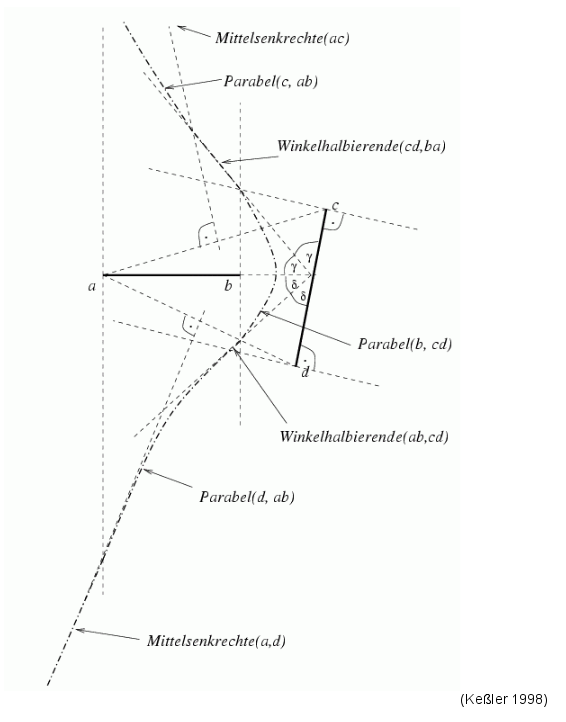
\includegraphics[width=0.5\textwidth]{bisektoren_zweier_strecken}} 
\end{figure} 
Quelle: uni-forst.gwdg.de/~wkurth/cb/html/alg\_v08b.pdf abgerufen am 28.05.2015 um 12:16 Uhr

\subsection*{Zusammenhängende Voronoi Regionen}

Sei $S$ eine Menge von Strecken und $l \in S$ eine Strecke und $d$ die Distanzfunktion.
Zu zeigen gilt: Das alle Punkt $x$ einer Voronoi Region  $VR(l, S)$ und alle Punkte einer Strecke von $\overline{x, y_x}$ in der VR liegt (dabei sei $y_x$ der nächste Punkt auf $l$).

Beweis: Wir wählen ein Punkt $a \in \overline{x, y_x}$ so das es im Abschluss einer VR $l'$ liegt. Dann wäre $d(l, z) \geq d(l', z)$ und $y_a$ sei der nächste Punkt auf der Strecke $l'$ so würde folgen

\begin{align}
d(l,x)=d(y_x, x) &= d(y_x,a)+d(a, x)\\
&= d(l, a) +  d(a, x) \\
&\geq d(l', a) +  d(a, x) \\
&= d(y_a, a) +  d(a, x) \geq d(y_a, x) \geq d(l', x)
\end{align} 

dies steht im Widerspruch zu unserer Annahme $x \in VR(l,S)$. $\square$ Daraus können wir direkt folgern das Voronoi Region von Strecken zusammenhängend Mengen sind.

\cite{Klein1997}

\subsection*{Aus wie vielen Ecken, Kanten und Zellen kann $VD(S)$ höchstens bestehen?}




\section*{Aufgabe 2 - Fortune-Sweep}


\begin{figure}[!htb]
    \subfigure[Schritt 1]{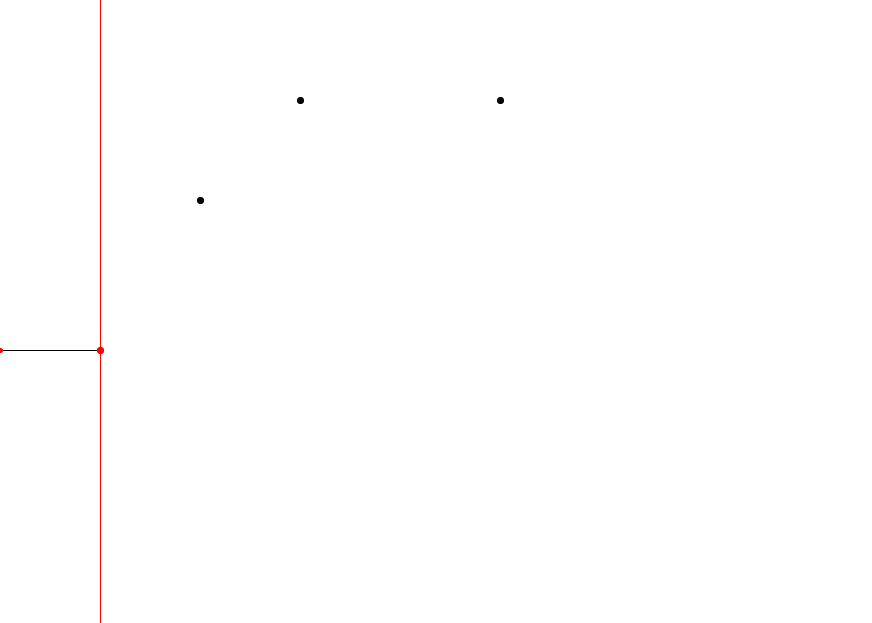
\includegraphics[width=0.5\textwidth]{01}} 
    \subfigure[Schritt 2]{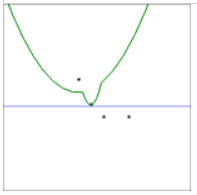
\includegraphics[width=0.5\textwidth]{02}} 
    \subfigure[Schritt 3]{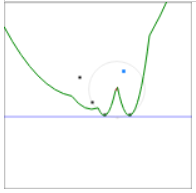
\includegraphics[width=0.5\textwidth]{03}} 
    \subfigure[Schritt 4]{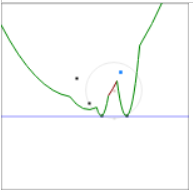
\includegraphics[width=0.5\textwidth]{04}} 
    \subfigure[Schritt 4]{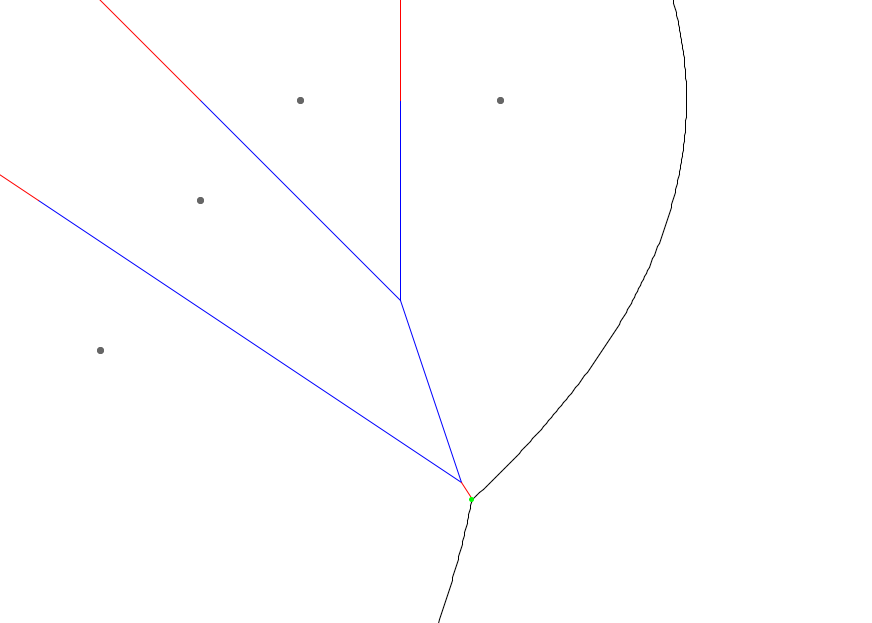
\includegraphics[width=0.5\textwidth]{05}} 
    \subfigure[Schritt 6]{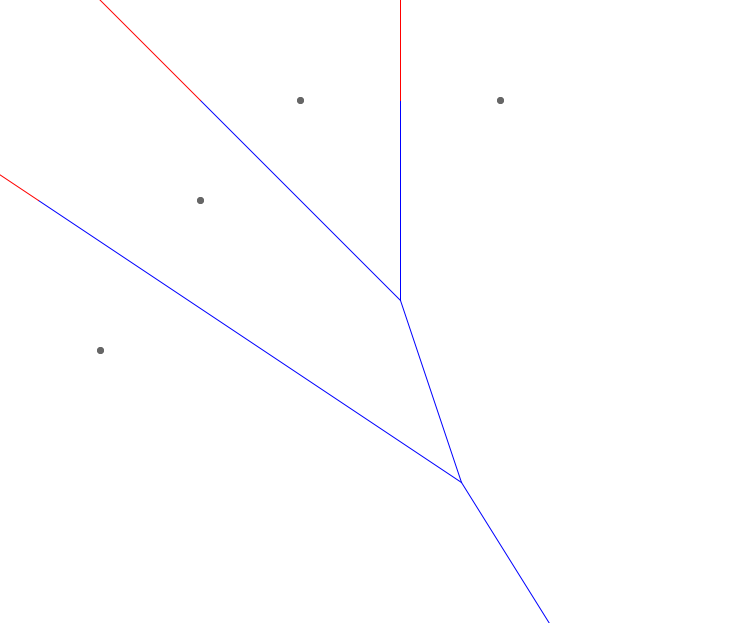
\includegraphics[width=0.5\textwidth]{06}} 
\end{figure} 


Der Fortune-Sweep-Line-Algorithmus lässt eine Linie $l$ in (den Abbildungen eine rot vertikale Linie) von dem kleinsten bis zu größten x-Wert über die Punktmenge bewegen, dabei werden folgende Events behandelt:

\begin{itemize}
	\item zu b) Der erste Punkt $(0, 0)$ betrachtet und die sogenannte Beach Line wird um eine Parabel erweitert.
	\item zu c) Die Sweep-Line wird auf den nächsten Eventpunkt $(1, 2)$ vorgerückt. Die Beach Line wird um ein weitere Parabel erweitert.
	\item zu d) Das gleiche passiert beim Punkt $(2, 3)$, die Beach Line wird um eine dritte Parabel erweitert. Der Schnitt Punkt der ersten beiden Parabeln zeigt schon eine Kante zwischen den beiden Voronoi Region (0, 0) und (1, 2), wobei der Voronoi Knoten noch nicht definiert ist.
	\item zu e) Der letzte Punkte $(4, 3)$ wird in der Event Queue bearbeitet und die Beach Line wird um die letzte Parabel ergänzt.
	\item zu f) Leider wird aus der Visualisierung das erstellen der beiden Voronoi Knoten nicht deutlich aber es werden lediglich beim entfernen einer Beach Line Abschnittst ein Voronoi Knoten (VK) hinzugefügt und die damit verbunden Kanten. Der erste VK liegt bei $(3, 1)$ und der zweite VK bei $(3.5, -0.5)$
	\begin{itemize}
		\item	1. Kante: $(3, \infty)$, $(3, 1)$
		\item	2. Kante: $(-\infty, \infty)$, $(3, 1)$
		\item	3. Kante: $(3, 1)$, $(3.5, -0.5)$
		\item	4. Kante: $(3.5, -0.5)$, $(-\infty, \infty)$
		\item	5. Kante: $(3.5, -0.5)$, $(-\infty, -\infty)$, 
	\end{itemize}
	\item zu g) Das Voronoi Digramm besitzt insgesamt zwei Voronoi Knoten, fünf Voronoi Kanten und vier offene Voronoi Regionen.
\end{itemize}


\section*{Aufgabe 3 - Durchschnitt einfacher Polygone}

%Quelle: http://geomalgorithms.com/a09-_intersect-3.html



\end{document}

\bibliographystyle{plain}
\bibliography{blatt06}

